% Slides for 2024-08-20
\begin{frame}{Endpoint detection}
    \begin{enumerate}
        \item Estimate endpoints using PCA
        \item Classify as head/tail
        \item Use a separate heuristic for each to adjust
    \end{enumerate}
\end{frame}

\begin{frame}{Head/tail classification}
    \begin{columns}
        \begin{column}{0.7\textwidth}
            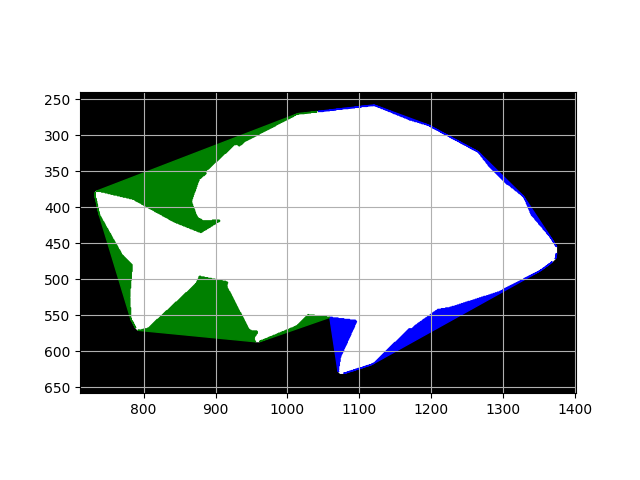
\includegraphics[height=0.7\textheight,width=0.7\textwidth,keepaspectratio]{images/fs_convex_difference.png}
        \end{column}
        \begin{column}{0.4\textwidth}

            \begin{itemize}
                \item Old alg: 125/138
                \item New alg: 138/138
                \item 100\%!
            \end{itemize}
        \end{column}
    \end{columns}
\end{frame}

\begin{frame}{Head point correction}
    \centering
    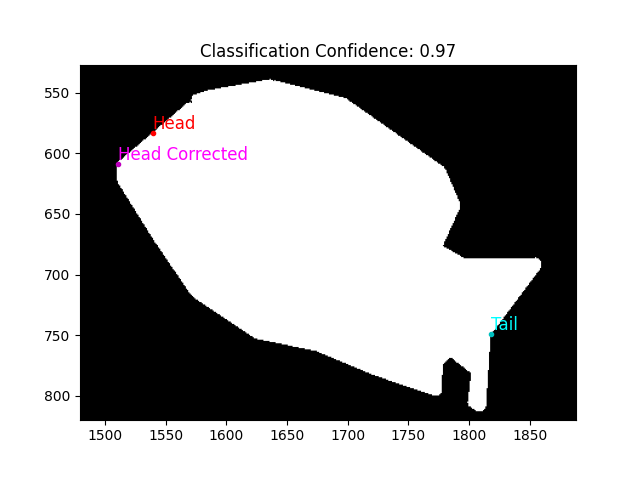
\includegraphics[height=0.6\textheight,width=0.6\textwidth,keepaspectratio]{images/fs_head_correction1.png}
    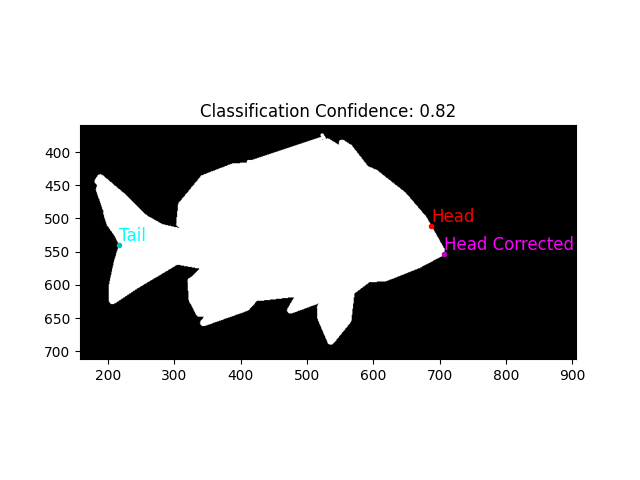
\includegraphics[height=0.6\textheight,width=0.6\textwidth,keepaspectratio]{images/fs_head_correction3.png}
\end{frame}

\begin{frame}{Head point correction}
    \centering
    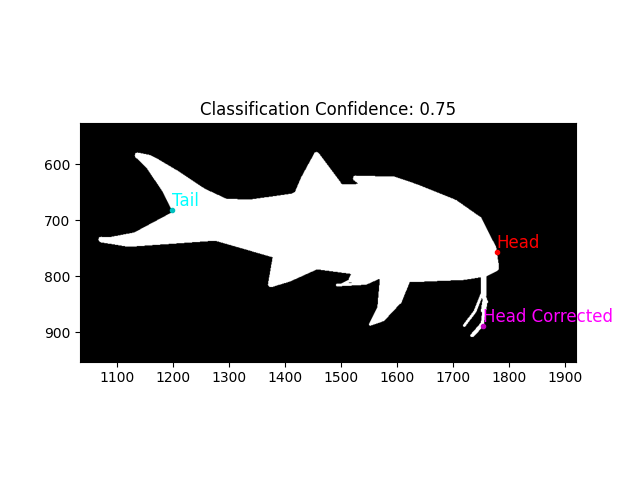
\includegraphics[height=0.6\textheight,width=0.6\textwidth,keepaspectratio]{images/fs_head_correction5.png}
    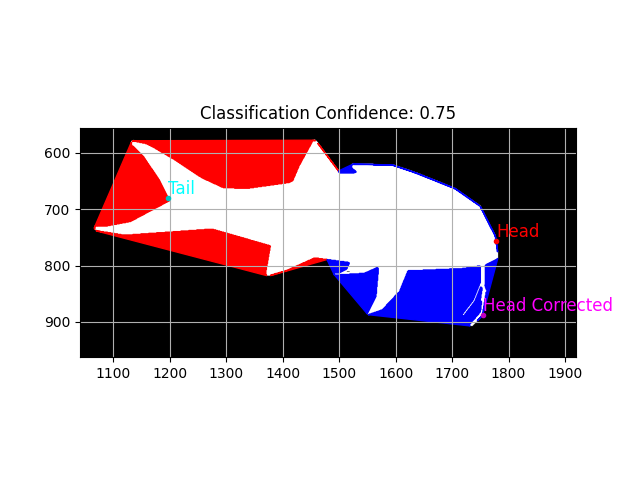
\includegraphics[height=0.6\textheight,width=0.6\textwidth,keepaspectratio]{images/fs_head_correction6.png}
\end{frame}